\chapter{関連研究}\label{chap:related}

本章では、本研究に関連する研究を分類し、それらの特徴や本研究との関連性について示す。

\newpage

\section{HumanComputation}\label{humancomputation}

コンピュータの計算能力だけでは解決できない問題を、人間の処理能力を計算資源として利用することによって解決する手法は、
ヒューマンコンピュテーション\cite{humancomputation}と呼ばれ、様々な研究が行なわれている。
現在のコンピュータの技術では、パターン認識など、高い精度で処理することが困難な分野が存在する。
こういった分野において、人間という柔軟な思考能力を持つ資源をコンピュータの代替として用いることで、
より高い精度の処理を実現することが可能である。

\paragraph{reCAPTCHA}\label{recaptcha}

\mbox{}

コンピュータの文字認識能力では処理しきれない文字の認識を人間に実行させるreCAPTCHA\cite{recaptcha}は、
人間かコンピュータかを判別するために文字認識をさせるCAPTCHA\cite{captcha}を応用したものである。
reCAPTCHAでは、人間に2種類の単語が書かれた画像が提示され、書かれている文字を入力させる。
片方の画像は文字認識がされており、書かれている内容がわかっている。
もう片方の画像は文字認識されていないもので、人間に認識させることでその答えを学習させる。
人間かコンピュータかの判別を行いつつ、人間に未認識の文字の認識作業に協力してもらうことができる仕組みである。

\begin{figure}[htbp]
  \begin{center}
  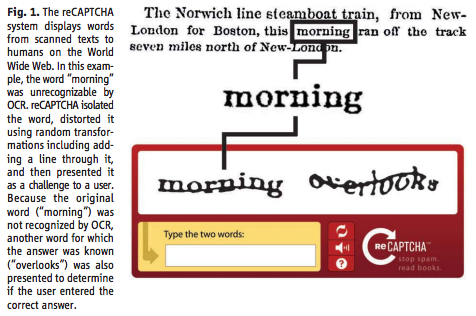
\includegraphics[width=.5\linewidth,bb=0 0 476 316]{images/recaptcha.png}
  \end{center}
  \caption{reCAPTCHA}
  \label{fig:recaptcha}
\end{figure}

\paragraph{Duolingo}\label{duolingo}

\mbox{}

Duolingo\cite{duolingo}は、一部のユーザの言語学習における翻訳作業を利用して、
ウェブサイトや文書の翻訳を行うアプリケーションである。
言語翻訳のための計算資源として人間を利用している。
言語学習自体もゲーミフィケーションを活用したものとなっており、翻訳作業しているということは隠蔽された形で語学学習できる。

\paragraph{Vizwiz}\label{vizwiz}

\mbox{}

人間を物体認識エンジンとして利用することのできるアプリケーションがVizwiz\cite{vizwiz}である。
アプリ利用者は認識したい物体をカメラで撮影し、質問内容などを録音して送る。
画像に対する質問はインターネットを介した人間に依頼される。
依頼された人間が応答し、その結果を返すことによって、アプリ利用者は答えを知ることが出来る。

\paragraph{Soylent}\label{soylent}

\mbox{}

Soylent\cite{soylent}は、文章の校正をインターネットを介した人間の力を利用して行うソフトウェアである。
文章の校正に関する多くの作業は、人間のほうが得意な作業となっている。
文章を意味が通じる状態を維持して短くすることや
文法的に正しくても意味の通じない文章を意味が通じるように変換する機能、
文脈に合った画像を探し出す機能などを人間に依頼することで実現している。

\paragraph{CrowdDB}\label{crowddb}

\mbox{}

計算機だけでは処理が困難なクエリに対して、人間を用いることで返答可能にする仕組みとして、
CrowdDB\cite{crowddb}が提案されている。
CrowdSQLという、SQLを拡張したものが記述言語として使われる。
CrowdSQLで書かれたクエリはクラウドソーシングされ、人間によって解釈され処理される。
また、結果はCrowdTableという形で、テーブルとして提供される。

\paragraph{Realitime-Captioning}\label{realitime-captioning}

\mbox{}

Laseckiら\cite{realtime-captioning}は、スピーチの動画等にリアルタイムでキャプションを付与するためのエンジンとして
人間を利用する手法を提案している。
通常、リアルタイムのキャプション付けに熟練した人間でないと出来なかった作業を、
非熟練の人間に複数人用意し、スピーチ動画を少しづつキャプション付けさせ、最終的に結合することで実現させている。

\section{CrowdSourcing}\label{crowdsourcing}

インターネットを介して不特定多数の人間に仕事を依頼する仕組みはクラウドソーシングと呼ばれ、近年注目を浴びている。
クラウドソーシングとは、業務の一部を外部に委託することを示すアウトソーシングという言葉を改変した造語である\cite{riseofcrowdsourcing}。
インターネットを介した不特定多数の人間たち(crowd)に仕事をアウトソースすることから、crowdsourcingと呼ぶ。
非常に安価で、かつ、必要な人員をすぐに確保して仕事依頼が可能である。
近年では、Amazon Mechanical
Turk\cite{amt}(以降MTurk)等のクラウドソーシングプラットフォームが登場してきたことによって
多くの利用例が生まれている。
クラウドソーシング分野の研究では、ヒューマンコンピュテーションの概念をクラウドソーシングを利用することで
大規模な人力処理を実現させている。

本節では、クラウドソーシングをより便利に扱えるようにするシステムの研究事例について紹介する。

\paragraph{Turkit}\label{turkit}

\mbox{}

Littleらは、MTurkをプログラムから簡単に利用するためのツールキットであるTurkit\cite{turkit}を提案している。
Turkitでは、通常のプログラミング記法と同じような記法でタスクをクラウドソーシングすることができる(図\ref{fig:turkit})。
また、クラウドソーシングによる処理結果の保存をしておくことで、その後の処理でプログラム実行に失敗しても
再度クラウドソーシングに処理依頼をするのではなく、保存済みの結果を元にプログラムを再度実行できるような仕組み
であるthe crash-and-return プログラミングモデルを提唱している。
可能な限り従来のプログラミング記法を崩さずに人力処理を組み込むことを目的としており、本研究と類似している。
本研究における提案手法は、クラウドソーシング処理を前提としておらず、特定の個人に対する指示を実現するものである。
Turkitでは特定個人に対する処理依頼を記述することはできない。

\begin{figure}[htbp]
  \begin{center}
  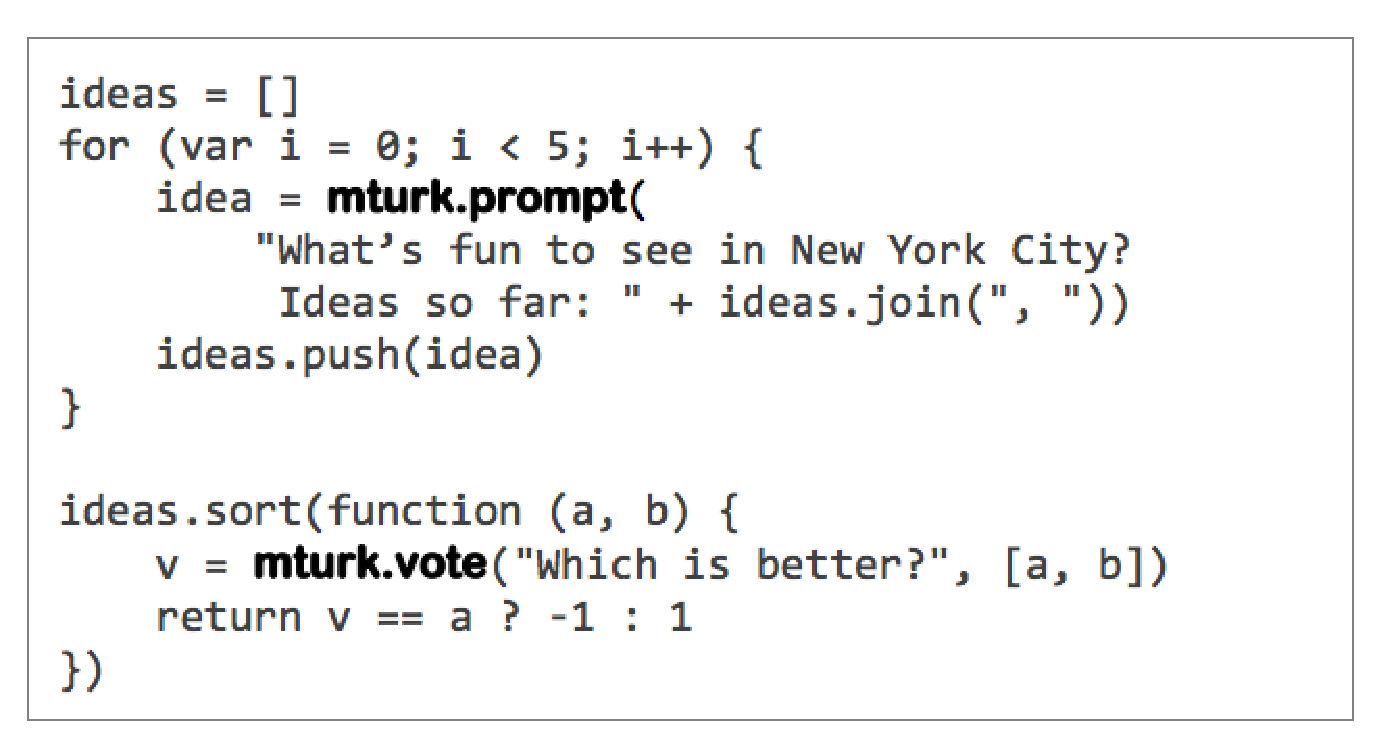
\includegraphics[width=.6\linewidth]{images/turkit.eps}
  \end{center}
  \caption{Turkit}
  \label{fig:turkit}
\end{figure}

\paragraph{Automan}\label{automan}

\mbox{}

Barowyらは、Automan\cite{automan}というプログラミング言語Scala上で動作するDomain
Specific Languageを提案した。
可能な限り通常のプログラミング記法を崩さずにクラウドソーシングを活用した人力処理を組み込むことを目的としており、
クラウドソーシングによる計算とコンピュータによる計算を統合したCrowdProgrammingを提案している。
また、回答の品質管理機能やタスクのスケジューリング、予算の配分等に関する機能を持つ。
本研究における目的は人間と計算機への指示を融合させたプログラミングを実現させることとなっており、
Barowyらが提唱したCrowdProgrammingと目的が類似している。

\begin{figure}[htbp]
  \begin{center}
  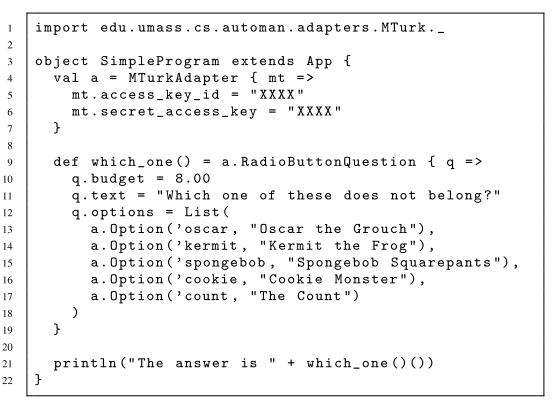
\includegraphics[width=.6\linewidth,bb=0 0 552 404]{images/automan.png}
  \end{center}
  \caption{Automan}
  \label{fig:automan}
\end{figure}

\paragraph{Cylog / Crowd4U}\label{cylog-crowd4u}

\mbox{}

Morishimaらは、人間と計算機の知の融合を目指した環境として、Cylog\cite{cylog}というDatalog\footnote{http://docs.racket-lang.org/datalog/}に類似した構文規則を持った
プログラミング言語と、その実行基盤であるCrowd4U\footnote{http://crowd4u.org/}を提案している。
Cylogでは人間を合理的に動くデータソースとして定義し、プログラム上で利用する。
類似した文法で人間と計算機の双方への命令を記述できる。
また、Crowd4Uという専用の実行基盤も実装している。

本研究では、クラウドソーシングそのものを利用していない。
また、Cylogでは人間をデータソースとして利用するが、
本研究では人間はデータソースに限らず、汎用な処理の実行対象として利用する。

\paragraph{CrowdForge}\label{crowdforge}

\mbox{}

Kitturら\cite{crowdforge}は、複雑な仕事をクラウドソーシング上で実現するための仕組みとして
CrowdForgeというシステムを提案している。
CrowdForgeはMapReduceの仕組みをクラウドソーシングに適応させた。
複雑な仕事を適切な大きさに分割し実行させ、最終的には結合させる機能を実装している。

\begin{figure}[htbp]
  \begin{center}
  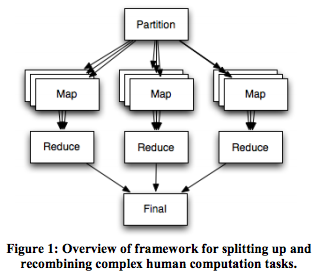
\includegraphics[width=.6\linewidth,bb=0 0 318 276]{images/crowdforge.png}
  \end{center}
  \caption{CrowdForge}
  \label{fig:crowdforge}
\end{figure}

\paragraph{Community Based
Crowdsourcing}\label{community-based-crowdsourcing}

\mbox{}

クラウドワーカーをある指標ごとにまとめたグループをコミュニティと呼び、
そのコミュニティの人たち及びコミュニティを横断したクラウドソーシングの仕組みについて提案している\cite{community-based-crowdsourcing}。
コミュニティは動的に変更することができるなど、柔軟にその構成を変化させることが出来る。

\section{Social Computing}\label{social-computing}

コンピュータ・ネットワーク上における群衆の様々な行動や叡智をフィードバックデータとして
システムに組み込み活用していくことはソーシャルコンピューティングと呼ばれている。
例えば、群衆による叡智が集められた情報をまとめるためのプラットフォームとしてはWiki\cite{wiki-way}が存在する。
Wikiの具体的なシステム例で有名なWebサービスがWikipedia\footnote{http://wikipedia.org}である。
また、人々が作るwebページのリンク関係からWebページの重要度を算出するアルゴリズムとしては、PageRank\cite{pagerank}が存在する。
PageRankは検索サービスのGoogle\footnote{https://google.com}で利用されている。
群衆の嗜好情報等を蓄積し、個人間の嗜好等の類似度から情報の推薦等を行う手法は協調フィルタリングと呼ばれる\cite{collaborative-filtering}。
主に商品の推薦システムなどにおいて利用されることが多い。

このように、インターネットを介した群衆の叡智を利用してシステムもしくはそのコンテンツを改良していく仕組みは
非常に有用で、多くのWebサービスに活かされている。
次に、特に本研究と関連するソーシャルコンピューティングシステムの事例を紹介する。

\paragraph{The Dog Programming
Language}\label{the-dog-programming-language}

\mbox{}

Webアプリケーションにおけるユーザとのインタラクションの記述に特化したプログラミング言語として、Dog\cite{dog}が提唱されている。
本研究も、人とのインタラクションの記述に特化したものであり、類似している。
DogはWebアプリケーションの実装時によくあるユーザとのインタラクションの記述に特化したものであるが、
本研究は人間を計算資源として様々な処理の実行指示を送るための仕組みである。

\begin{figure}[htbp]
  \begin{center}
  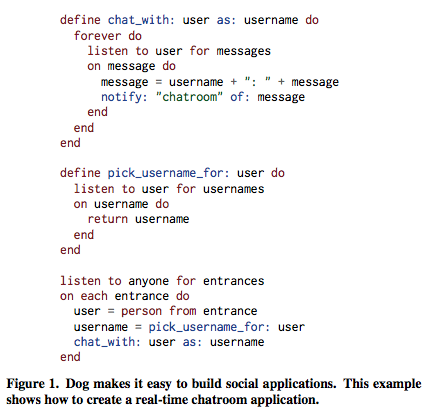
\includegraphics[width=.6\linewidth,bb=0 0 426 414]{images/dog.png}
  \end{center}
  \caption{The Dog Programming Language}
  \label{fig:dog}
\end{figure}

\paragraph{The Jabberwocky Programming Environment for Structured Social
Computing}\label{the-jabberwocky-programming-environment-for-structured-social-computing}

\mbox{}

Ahmadらは、Jabberwockyというソーシャルコンピューティングのためのプログラミング環境を提案している\cite{jabberwocky}。
Jabberwockyは、様々なクラウドソーシングプラットフォームを統合して管理できるDormouseと、
Dormousとのインタラクションに特化したDog,
MapReduceを人力処理に適応したManReduceから構成される。

\paragraph{Personal APIs As an Enabler for Designing and Implementing
People As Social
Machines}\label{personal-apis-as-an-enabler-for-designing-and-implementing-people-as-social-machines}

\mbox{}

Buregioらは、Social
Machine\cite{social-machines}という研究分野について整理し、その具体的な例として
Personal APIs\cite{personal-api}を提唱している。 Social
Machineは、SocialSoftwareとPeople as Computational Units、Software as
Sociable Entitiesの 3つの領域が重なり合った研究領域である。
この領域において、人間にAPIを付与し、情報にアクセス可能にするという仕組みが、Personal
APIsという概念である。
このAPIを通して、例えばカレンダー情報等にアクセスする。
実装はなく、概念の提唱にとどまっている。

\section{Human as Sensor}\label{human-as-sensor}

人間をセンサー代わりにしたり、人間が持つスマートフォン等のデバイスのセンサーを利用する手法はHuman
as Sensorや参加型センシング\cite{participatory-sensing}と呼ばれる。
ユビキタスコンピューティング\cite{weiser1991computer}などの研究分野において、こういった手法が多く研究されている。
その事例を以下に紹介する。

\paragraph{PRISM}\label{prism}

\mbox{}

Dasらは、PRISM\cite{prism}というスマートフォンを利用した参加型センシング実現のためのプラットフォームを提案している。
参加型センシングをより現実的に実行可能にするためには、セキュリティやスケーラビリティのバランスが取れた
より使いやすいプラットフォームが必要とされているとし、そのためのプラットフォームとしてPRISMを提案している。

\begin{figure}[htbp]
  \begin{center}
  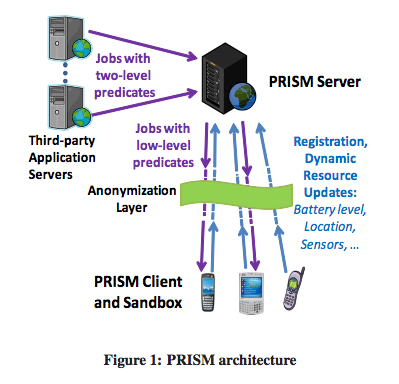
\includegraphics[width=.6\linewidth,bb=0 0 399 384]{images/prism.png}
  \end{center}
  \caption{PRISM: Platform for Remote Sensing using Smartphones}
  \label{fig:prism}
\end{figure}

\paragraph{Moboq}\label{moboq}

\mbox{}

Liuらは、リアルタイムな位置情報ベースQ\&AサービスのMoboQを提案している\cite{moboq}。
マイクロブログサービスを利用したシステムであり、指定した場所にいる人間を対象とした参加型センシングシステムとなっている。

\section{Human as Actuator}\label{human-as-actuator}

アクチュエータ技術は進歩しているが、未だに人間のような汎用的に実世界に干渉できる装置はない。
そこで、人間をアクチュエータの代替として利用し動かす、つまり、人間とロボットの協調によって問題を解決しようという研究がある。

\paragraph{HapticTurk}\label{hapticturk}

\mbox{}

Hapticturk\cite{hapticturk}は、人間をモーションプラットフォームのモーターやメカニカル機構の代わりに使うことによって、
モーションプラットフォームの動きを再現するというものである。
人間への動きの指示はスマートフォンなどを経由して行なわれる。
人間をアクチュエータの代わりに利用するといった点において、本研究と類似している。
本研究では、その用途をアクチュエータに限ったものではない。
また、プログラム上で汎用的に利用可能である。
Hapticturkでは、ゲームにその用途を限定している。

\begin{figure}[htbp]
  \begin{center}
  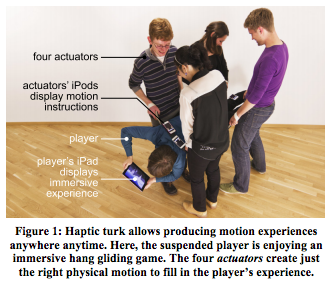
\includegraphics[width=.6\linewidth,bb=0 0 332 281]{images/hapticturk.png}
  \end{center}
  \caption{Hapticturk}
  \label{fig:hapticturk}
\end{figure}

\paragraph{Sharedo}\label{sharedo}

\mbox{}

加藤ら\cite{sharedo}は、ロボットや様々なソフトウェアエージェントと人間のタスクを
同列に記述可能なタスク共有アプリケーションを提案している。
タスクの実行主体は人間でもコンピュータでも良いようになっており、人間とコンピュータは処理実行対象として
同等となっている。 また、Human
Actuation等の概念についても論文内において触れられている。
処理実行対象を選ばないという点において、本研究と類似している。

\begin{figure}[htbp]
  \begin{center}
  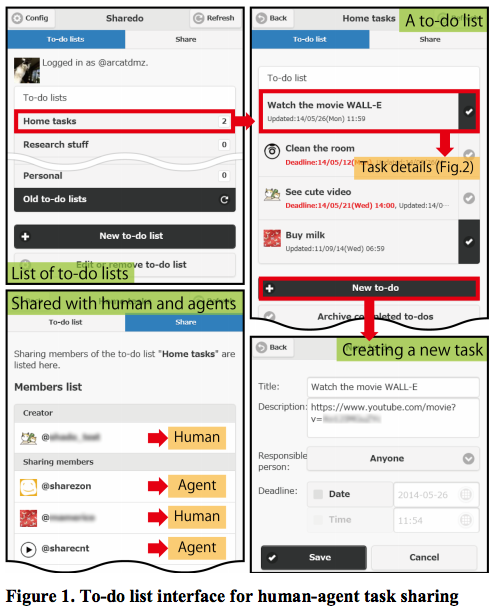
\includegraphics[width=.5\linewidth,bb=0 0 497 611]{images/sharedo.png}
  \end{center}
  \caption{Sharedo}
  \label{fig:sharedo}
\end{figure}

\paragraph{グラフィカルデータフローによる調理レシピプログラミング言語の提案}\label{ux30b0ux30e9ux30d5ux30a3ux30abux30ebux30c7ux30fcux30bfux30d5ux30edux30fcux306bux3088ux308bux8abfux7406ux30ecux30b7ux30d4ux30d7ux30edux30b0ux30e9ux30dfux30f3ux30b0ux8a00ux8a9eux306eux63d0ux6848}

\mbox{}

吉川らは調理レシピを記述するためのデータフロープログラミング言語を提案している\cite{recipe-programming}。
料理レシピをグラフィカルなデータフローで記述する。
料理レシピプログラムは、コンピュータではなく人間が実行するためのものである。
本研究のように、人間がプログラムからの指示を実行することを前提としたものとなっている。

\paragraph{Cooky}\label{cooky}

\mbox{}

Sugiuraらは、人間とロボットが協調して調理をするシステムCooky\cite{cooky}を提案している。
料理支援ロボットと人とロボットが共有可能な調理器具やキッチン、調理手順を記述するシステムから成り立っている。
調理手順記述システムでは、人間とロボット双方の処理を分けて記述することができる。
人間とロボットが協調して作業を実行していくモデルは、本研究が実現したい目標とも似ている。

\begin{figure}[htbp]
  \begin{center}
  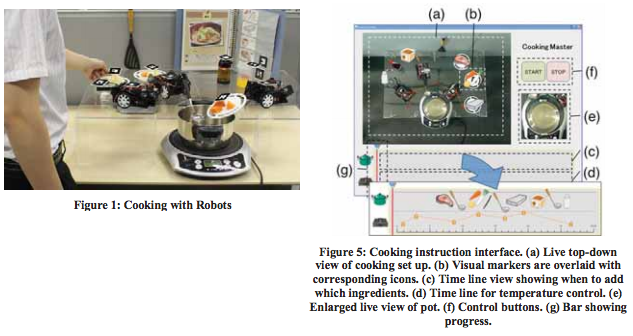
\includegraphics[width=.6\linewidth,bb=0 0 633 336]{images/cooky.png}
  \end{center}
  \caption{Cooky}
  \label{fig:cooky}
\end{figure}

\section{Workflow Programming}\label{workflow-programming}

仕事などにおけるプロセスを文書などによってパターンとして規定し、検証や再利用しやすくするためのものとして
ワークフローというものがある。
このワークフローを構築するための仕組みが複数存在する。

YAWL\cite{yawl}は、ワークフローやビジネス・プロセスを記述するためのワークフロー記述言語である。
類似のものとしては、XPDL(XML Process Definition
Language)\cite{xpdl}が存在する。
これらのワークフロー記述言語を実行するワークフローエンジンと呼ばれるソフトウェアも多く存在する。
ワークフロー記述言語は、ワークフローを記述するものである。
プログラムによる処理を記述することはできない。

また、X-point\footnote{https://www.atled.jp/xpoint/}や
questetra\footnote{http://www.questetra.com/ja/}といった
ワークフロー記述・実行のためのWebサービスも存在する。
